% kapitel4.tex
\chapter{Implementation}
\label{chapter:realisierung}
Now, that a basic abstract model is designed a implementation in Cinco can be made. Like shown in figure \ref{fig:ModelLayers} a separation of the layers will result in four different \gls{mgl} files. This leads to four different models which have to be combined with the feature already introduced called prime references. For each of them an example will be appended to clarify the proper handling and to understand the meaning of each modeling step.
\section{MGL}
Even though the style definitions using \gls{msl} are very minimal in this case the focus is set on the model \gls{mgl} files.
First of all the sensor layer should be described as the rest of the model is based on this step.
\subsection{Sensor}
The one and only node without any child nodes is called metric and describes a metric like introduced in chapter \ref{chapter:grundlagen}. 
\begin{listing}[H]
	\begin{minted}{\mgllexer}
		@style(sensorMetric, "${label}")
		@icon("src/main/resources/icons/file-export-solid.16.png")
		node Metric {
			outgoingEdges (ContainedBy)
			attr EString as label := ""
		}
	\end{minted}
	\caption{Impl. of Metric Node}
	\label{lst:nodeMetric}
\end{listing}
As shown a metric has a label describing its function like power or humidity. It has to represent the names of the metrics which are exported through the Prometheus interface. A metric can have multiple connections to different sensors but not more than one connection to a sensor.

Senors combine these metrics (line 4, figure \ref{fig:CodeSensorDevice}) into a group of exportable data. This step is done and needed for modeling real world sensor devices. This devices can be reused everywhere in the project since it is an abstract and not a concrete instance of the device holding configuration or being used. 

Attributes like a name and a specific icon  can also be edited. The names for the sensors are used to keep them apart. For a better \gls{ui} experience it is possible to select a symbol from a preselected set of icons to show up in the node. This makes it easier to get a faster coordination in bigger networks. This feature gets enabled by the $SensorIconValueProvider$ class linked with the $@possibleValuesProvider$ annotation (listing \ref{lst:classSensorIconValueProvider}).
\begin{listing}[H]
	\begin{minted}{\mgllexer}
	@style(sensorDevice, "${name}")
	@palette("DeviceDefinition")
	node DeviceDefinition {
		incomingEdges (ContainedBy)
		attr EString as name := ""
		@possibleValuesProvider("dev.schoki.metricarchitect.provider .SensorIconValueProvider")
		attr EString as icon
	}	
	\end{minted}
	\caption{Impl. of DeviceDefinition Node}
	\label{fig:CodeSensorDevice}
\end{listing}
For a faster access to the tooling some presets are implemented setting a predefined icon.
\subsection{Floor}
The modeled sensor using the previous \gls{mgl} definition can now be instantiated and configured. This can be achieved using the node $Device$. Via prime reference a link to a $DeviceDefinition$ is created (lines 4-6, \ref{fig:CodeSensorDeviceInstance}). Since it is not a specific real world device a symbolic name and a \gls{url} has to be set. The name is only used for better readability and the \gls{url} is essential. It will be generated into the Prometheus configuration for the deployment. Every node of this type corresponds to a device observed by Prometheus. 

To create a improved overview and handling a simple grouping is also implemented. This can be done by using the $Filter$ edges from the $Device$ to a $DeviceGroup$. For example it is possible to combine all power sockets or lights to one node to make them better accessible in the later steps. 

\begin{listing}[H]
	\begin{minted}{\mgllexer}
	@style(sensorInFloorModel, "${name}")
	@icon('src/main/resources/icons/bolt-solid.16.png')
	node Device {
		@pvLabel (name)
		@pvFileExtension ("sensor")
		prime SensorModel::DeviceDefinition as sensor
		outgoingEdges (GroupBy)
		attr EString as name := "DeviceName"
		attr EString as url := "localhost:8080"
	}	
	\end{minted}
	\caption{Impl. of Device Node}
	\label{fig:CodeSensorDeviceInstance}
\end{listing}

The generators for the needed configurations will follow later (see \autoref{}). For a better understanding where the devices are in the real world it is possible to use the $FloorImage$ node. It has only one variable which can be set to the path of an image inside the project relative to the root. Preferably a floor plan is used. With this creating device instances without forgetting which node matches with which real world device can be easily achieved.

\subsection{Grafana}

Using the previous devices and device groups it is no possible to model the Grafana configuration. Instead, it start by creating a new node via prime reference which is than embedded into a $GraphQueryForGroup$ or for non groups $GraphQueryForDevice$ node. Both wield the same information but it is necessary to distinguish between them because the generators act differently while processing these nodes. Since this node only works as a connection to the floor \gls{mgl} it does not contain more information. 

\begin{listing}[H]
	\begin{minted}{\mgllexer}
		@style(graphQueryForGroup, "${deviceGroup.name}")
		@icon('src/main/resources/icons/chart-line-solid.16.png')
		node GraphQueryForGroup {
			@pvLabel (name)
			@pvFileExtension ("floor")
			prime FloorModel::DeviceGroup as deviceGroup
			outgoingEdges (GraphQueryToPanel)
		}
	\end{minted}
\end{listing}

Due to this layer covering the Grafana configuration \gls{promql} queries are an essential part of it. The outgoing edge $GraphQueryToPanel$ covers a rich set of possible queries but not the overall features. It is the part of the model which describes the derived \gls{promql} query the most. Like already mentioned in subsection \ref{subsec:promql} there are different parameters to set. It is necessary to keep up to the right syntax, because the values for the variables are unchecked strings. The fields $timespan$, $timeresolution$ and $offset$ (line 6-8, listing \ref{lst:GraphQueryToPanel}) has to follow the roles for duration notation (page \pageref{lst:promql_vector}, figure \ref{lst:promql_vector}). All connected devices either connect via device groups or can directly have many different metrics. Since it does not make sense to show not compatible metrics in the same graph, like power and humidity, a value provider filters all common metrics of the devices. 

\begin{listing}[H]
	\begin{minted}{\mgllexer}
@style(simpleArrow)
edge GraphQueryToPanel {
	@possibleValuesProvider("dev.schoki.metricarchitect.provider .FilterValueProvider")
	attr EString as filter
	attr Aggregation as function := "none"
	attr EString as offset
	attr EString as timespan
	attr EString as timeresolution
}
	\end{minted}
	\caption{Impl. of the Edge connecting GraphQueryByGroup/GraphQueryByDevice to a Panel symbolizing a PromQL Query}
	\label{lst:GraphQueryToPanel}
\end{listing}

The $FilterValueProvider$ class (page \pageref{lst:classFilterValueProvider}, listing \ref{lst:classFilterValueProvider}) has to take into consideration that there are $GraphQueryByGroup$ and $GraphQueryByGroup$. This is done by a simple type checking in runtime with the java $instanceof$ keyword. Using this way a drop down menu will only allow valid metrics to be used.

Lastly an aggregation operator has to be selected. The default is $none$. This is not a function implemented by \gls{promql} but it is used as a keyword in this project for doing nothing, meaning there will not be a function around the generated query. The original \gls{promql} has many different functions and as already said, for this project only some of them are implemented. 

\begin{center}
	none | sum | min | max | avg | group | stddev | stdvar | count | count\_values | bottomk | topk  | quantile
\end{center}

It can be easily expanded but for a simple proof of concept the set is sufficient. These edges can than be merged to a $Panel$ node. At this state it does not have specific attributes. Yet, it can technically have all needed properties which can be used for setting up a Grafana panel. This could be width and height, position in x and y coordinates, graph style and so on.

With the non specific edge $PanelToDashboard$ a connection to the last node in this \gls{mgl} file can be established. The final node is the $Dashboard$ node. It is not very interesting but it has a name which is used by Grafana as the shown identifier. Additionally a unique id has to be set to ensure the correct functionality of Grafana. This is done by using the $@postCreate$ annotation (line 3, listing \ref{lst:nodeDashboard}) and a proper class for it. The class $DashboardPostCreateSetUniqueId$ creates a random string which will be set as $internal\_id$. This value is nothing the developer has to take care of and plays only an important role for the generator.

\begin{listing}
	\begin{minted}{\mgllexer}
	@style(dashboard, "${name}")
	@icon('src/main/resources/icons/list-alt-regular.16.png')
	@postCreate('dev.schoki.metricarchitect.hooks.grafanamodel.DashboardPostCreateSetUniqueId')
	node Dashboard {
		incomingEdges (PanelToDashboard)
		attr EString as name := ""
		final unique attr EString as internal_id := " " 
	}
	\end{minted}
	\caption{Impl. of Dashboard Node}
	\label{lst:nodeDashboard}
\end{listing}
\subsection{Project}
The Project layer was added to have a better overview. It can contain different information which can be possibly needed for better management. Extensions like adding options for the docker deployment or specific settings for Grafana and Prometheus could be added here in future work. Furthermore it is used as an entrypoint for the generators. 

The one and only node in this layer is the $GrafanaModel$ node which has a prime reference to a whole Grafana layer model file. It is possible to add multiple nodes.

Like already mentioned, this layer is the beginning for the generation process. A generator is appended with a $@generatable$ annotation. The class $ProjectGenerator$ therefor does all necessary steps. 

\begin{listing}[H]
	\begin{minted}{\mgllexer}
	
	@style("model/General.style")
	@primeviewer
	@generatable("dev.schoki.metricarchitect.codegen.ProjectGenerator","/src-gen/")
	graphModel ProjectModel {
		...
	}
	\end{minted}
	\caption{Impl. of ProjectModel Graph Model}
	\label{lst:modelProjectModel}
\end{listing}

\section{Example}
To wrap everything up and show how the different layers work with each other an example project will be set up. Multiple smart power sockets were used for this. In this case the Gosund SP1 will be used with a flashed firmware.
\begin{figure}[H]
	\centering
	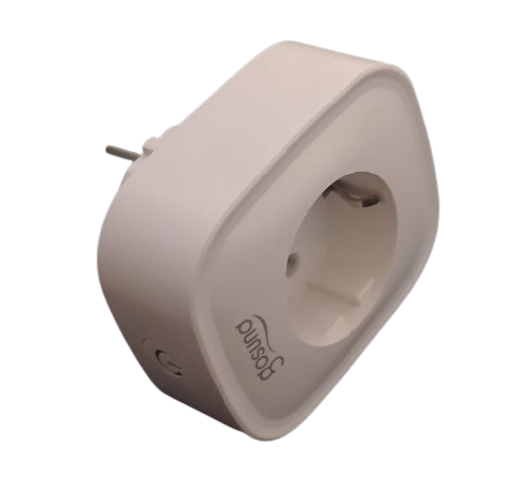
\includegraphics[width=4cm]{assets/images/gosund.png}
	\caption{Gosund SP1 Smart Power Socket}
\end{figure}
The open source project Tasmota \cite{tasmotawebsite} which is licensed under \gls{gpl3} is an alternative firmware for a huge amount of different \gls{iot} devices like lights, switches, curtains or power sockets like needed in this case.
With the version 8.5.1 which was released on 2nd October 2020 Tasmota gets optional support for Prometheus exports. 

Connecting to the correct \gls{url} under $/metrics$ will then return a well formatted Prometheus export ( see \ref{lst:exGosundExport} ).

\begin{listing}[H]
	\begin{minted}{text}
		# TYPE energy_voltage_volts gauge
		energy_voltage_volts 239
		# TYPE energy_current_amperes gauge
		energy_current_amperes 0.218
		# TYPE energy_power_active_watts gauge
		energy_power_active_watts 36
	\end{minted}
	\caption{Part of the Export of Gosund SP1 with Tasmota Firmware. Unimportant metrics are not shown.}
	\label{lst:exGosundExport}
\end{listing}

These three metrics are the one which should be modeled in the Cinco product. The metrics $energy\_voltage\_volts$, $energy\_current\_amperes$ and $energy\_power\_active\_watts$ has to be created using the metric node type. Additionally a new device definition is needed. In this case it will be named $tasmota\ ps$. Each of the created metrics needs than to be connected to the device definition.

\begin{figure}[H]
	\centering
	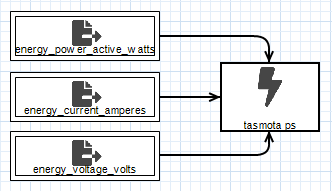
\includegraphics[width=.7\linewidth]{assets/images/sensorLayer}
	\caption{Modeled Sensor in the Sensor Layer}
\end{figure}

Based on this model the real world scenario will be created. It is not only important to know, that a sensor exist, it is also important to have some metadata of it. The position and ip are the needed ones here. Across two room four of these smart power sockets were placed. Two of them in the office and two more in the living room. Each of Bob and Alice computer is now monitored by such a smart socket. Additionally a \gls{hifi} audio system and the corresponding sub woofer in the living room are going to be observed. To make the handling easier a grouping is introduced. A group named $sound$ wields $hifi$ and $subwoofer$, group $computer$ has $bob$ and $alice$. The last group $all$ has each device connected to it. The floor plan was created in Sweet Home 3D is also open source and free to use. 

\begin{figure}[H]
	\centering
	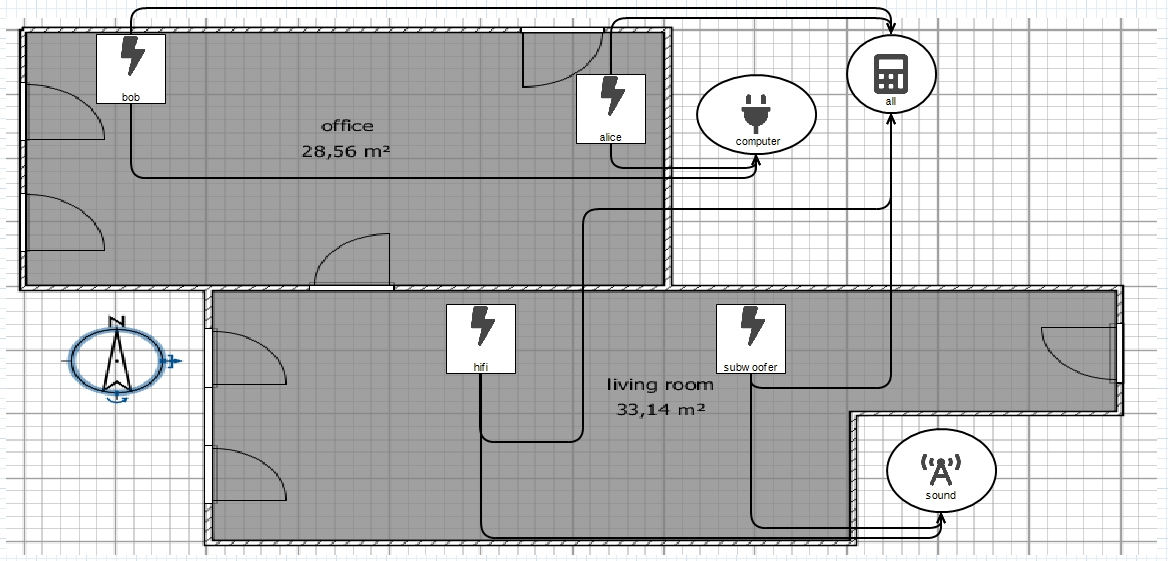
\includegraphics[width=\linewidth]{assets/images/floorLayer}
	\caption{Modeled Floor in the Floor Layer}
\end{figure}

After completing the translation of the upper scenario into the model the next step is to form the \gls{promql} queries and define which query goes in which panel. Afterwards the panels has to be grouped into dashboards. The most work has to be done configuring the edges from the device nodes to the panels.

From the floor layer the groups are included via prime references into the Grafana layer as seen on the left hand side in figure \ref{fig:modelGrafanaLayer}. From the $all$ node following connections are done:

\begin{itemize}
	\item Sum of $energy\_power\_active\_watts$ to power panel
	\item All $energy\_power\_active\_watts$ to power panel
	\item All $energy\_current\_amperes$ to current panel
 	\item All $energy\_voltage\_volts$ to voltage panel
\end{itemize}

This result in every power consumption shown in the panel view. As an addition the sum of all these values will be drawn. The panels for current and voltage does not contain any accumulated values but only the raw measured metrics. All three panels are then merged in the dashboard called $all$.

On the other side the group $sound$, combines the $hifi$ and $subwoofer$ device. The edges filters for each power, current and voltage. For a better overview for power and current the sum and for voltage the average will be calculated. 

The $groups$ dashboard has the panels which show the values of the group $sound$ and $computer$. Both power panels are both displayed in the power dashboard.

\begin{figure}[H]
	\centering 
	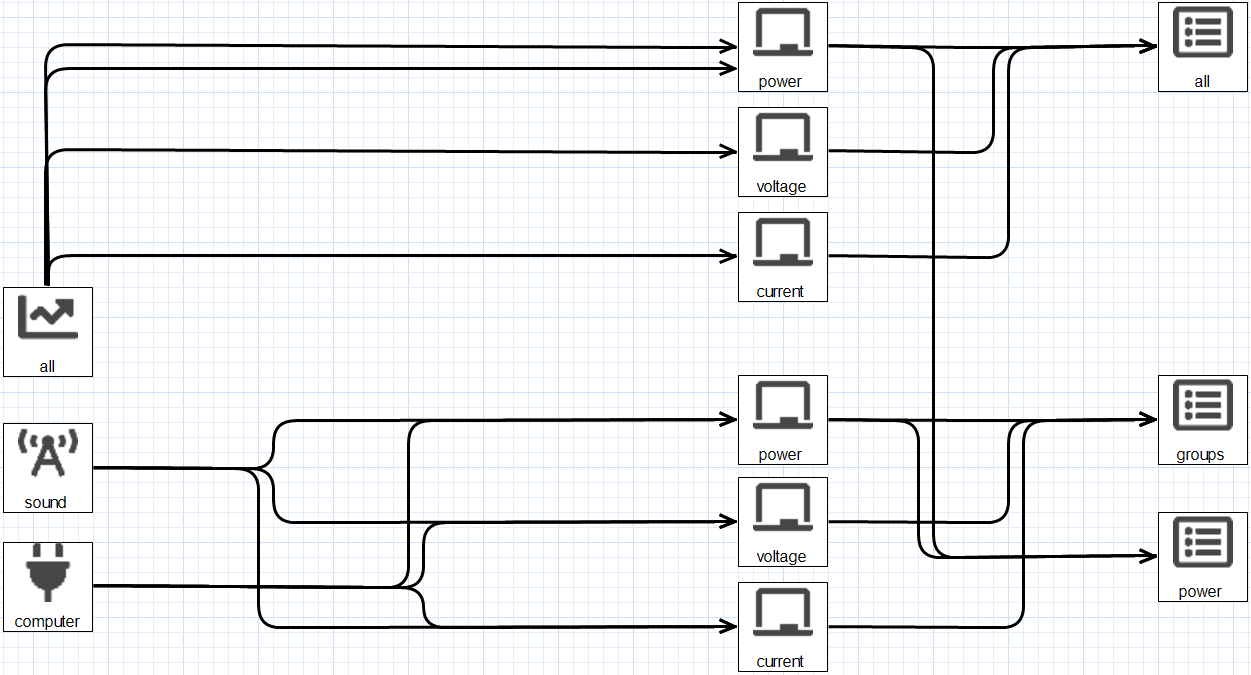
\includegraphics[width=\linewidth]{assets/images/grafanaLayer}
	\caption{Modeled Grafana in the Grafana Layer}
	\label{fig:modelGrafanaLayer}
\end{figure}

At the end the last layer for the project level is very minimal an just have one node with the name $Main$.

\begin{figure}[H]
	\centering
	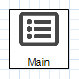
\includegraphics{assets/images/projectLayer}
	\caption{Modeled Project in the Project Layer}
\end{figure}

After generating this project the  deployment is very simple. Different configuration files are getting generated. For Prometheus the $prometheus.yml$ file is created. It has all information inside which are needed to listen to the sensors and grab their values for further processing. Therefor, Grafana need some more files. A file for the data source definition having all needed parameters for a valid connection between Prometheus and Grafana, a file $dashboards_config.yml$ has the meta information like organization name but also describes where Grafana can find the generated dashboard definitions. These definitions are also the last of the three components being generated. Panels used across multiple dashboards can not be created once and shared but they have to be generated multiple time and saved in each dashboard definition file.

For this the template functions of Xtend was heavily used as skeleton configuration files were extended using this feature. Simple tree traversing through the different layers of nodes was used to collect all needed data to finalize the configuration files. Additionally some helper functions were written for formatting and composing the gathered information. 

To make testing easier a $docker-compose.yml$ was created. It utilizes Docker and the Docker Compose~\cite{poulton2019docker} feature.  This allows a very fast startup and test of the generated project.

